\documentclass[11pt,a4paper]{article}

\usepackage[T1]{fontenc}
\usepackage[utf8]{inputenc}
\usepackage[spanish,es-tabla]{babel}
\usepackage{lmodern}
\usepackage{microtype}
\usepackage{geometry}
\usepackage{graphicx}
\usepackage{booktabs}
\usepackage{tabularx}
\usepackage{array}
\usepackage{amsmath,amssymb}
\usepackage{setspace}
\usepackage{caption}
\usepackage{float}
\usepackage{enumitem}
\usepackage{xcolor}
\usepackage{hyperref}

\geometry{margin=2.0cm, top=1.7cm, bottom=1.8cm}
\setstretch{1.05}
\setlength{\parskip}{0.25em}
\setlength{\parindent}{0pt}
\setlist[itemize]{leftmargin=1.2em, itemsep=0.1em, topsep=0.15em}
\setlist[enumerate]{leftmargin=1.2em, itemsep=0.1em, topsep=0.15em}
\captionsetup{font=footnotesize, labelfont=bf, skip=3pt}
\hypersetup{colorlinks=true, linkcolor=black, urlcolor=blue!50!black, citecolor=black}

\newcommand{\pregunta}[1]{\noindent\textbf{Pregunta.} #1\par}
\newcommand{\resultado}[1]{\noindent\textbf{Resultado.} #1\par}
\newcommand{\interpretacion}[1]{\noindent\textbf{Interpretación.} #1\par}
\newcommand{\verif}[1]{\noindent\small\textit{Verificación y límites.} #1\par}

\title{\bfseries Planificación de capacidad bajo incertidumbre\\
\large Reoptimización, compra de capacidad y compromiso robusto --- DataCare}
\author{Lorenzo Marquesini\\[0.25em]
\small Investigación Operativa --- Clase 04}
\date{}

\begin{document}
\vspace{-0.6em}
\maketitle
\vspace{-1.4em}

\begin{abstract}
\noindent
DataCare elige el mix trimestral de paquetes $A$ (automatización), $P$ (analítica predictiva) y $D$ (despliegue dedicado) sujeto a capacidad de ingeniería, especialistas y plataforma. Se resuelven tres LP continuos con OR-Tools (GLOP): plan base y sensibilidad; compra endógena de capacidad; plan robusto ante tres escenarios. Conclusión operativa: ingeniería y especialistas limitan el plan; conviene comprar a los precios actuales; comprometer el mix antes de conocer la capacidad cuesta $\approx 9$--$10\%$ del impacto potencial.
\end{abstract}

\noindent\textit{Unidades:} puntos de impacto y unidades de capacidad. Sin conversión monetaria.

%==============================================================================
\section{Qué limita el plan óptimo hoy}
%==============================================================================

\pregunta{¿Qué recursos restringen hoy el impacto máximo?}

\subsection*{Modelo}
\begin{equation}
\max Z = 72A + 95P + 120D
\end{equation}
\begin{align}
3A + 2P + 4D &\le 120 && \text{(Ingeniería)},\\
A + 3P + 2D &\le 80 && \text{(Especialistas)},\\
2A + P + 3D &\le 100 && \text{(Plataforma)},
\end{align}
con $0\le A\le 30$, $0\le P\le 25$, $0\le D\le 20$ (variables continuas).

\subsection*{Resultado}
\[
(A,P,D)\approx(5{,}71;\;11{,}43;\;20),\qquad Z\approx 3\,897{,}14.
\]
Ingeniería y especialistas: utilización $100\%$. Plataforma: holgura $\approx 17{,}14$ ($\approx 17\%$). $D$ en su tope de demanda. Precios sombra locales: $\approx 17{,}29$ (Ing), $\approx 20{,}14$ (Esp), $0$ (Plat).

\begin{figure}[H]
\centering
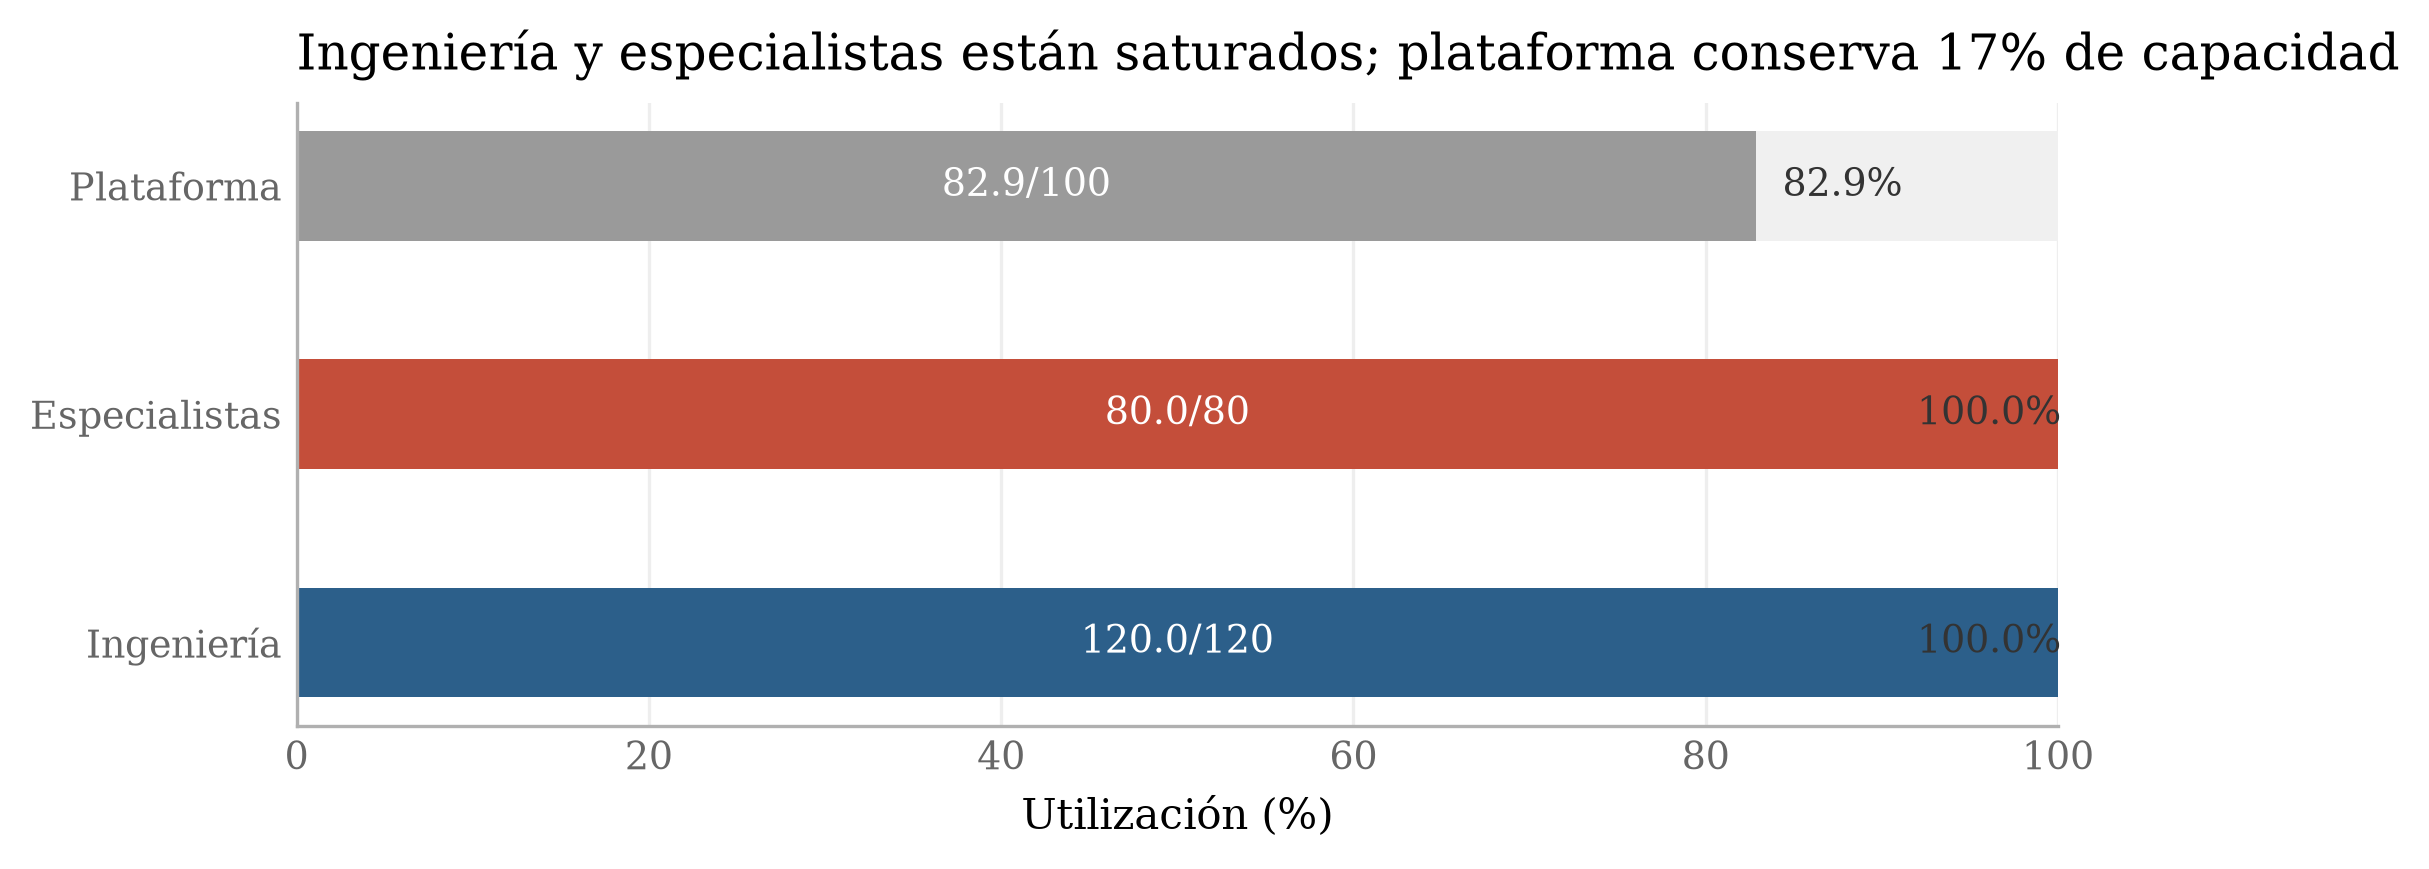
\includegraphics[width=0.80\textwidth]{report_assets/01_base_utilization.png}
\caption{Utilización en el plan base: saturación de ingeniería y especialistas.}
\label{fig:util}
\end{figure}

\interpretacion{Plataforma no es el cuello de botella. El margen de mejora está en ingeniería y, sobre todo, en especialistas.}

\subsection*{Sensibilidad continua (0--40\%)}

Al ampliar un recurso a la vez, el valor y el mix cambian de forma distinta (Figuras~\ref{fig:sens1} y~\ref{fig:sens2}).

\begin{figure}[H]
\centering
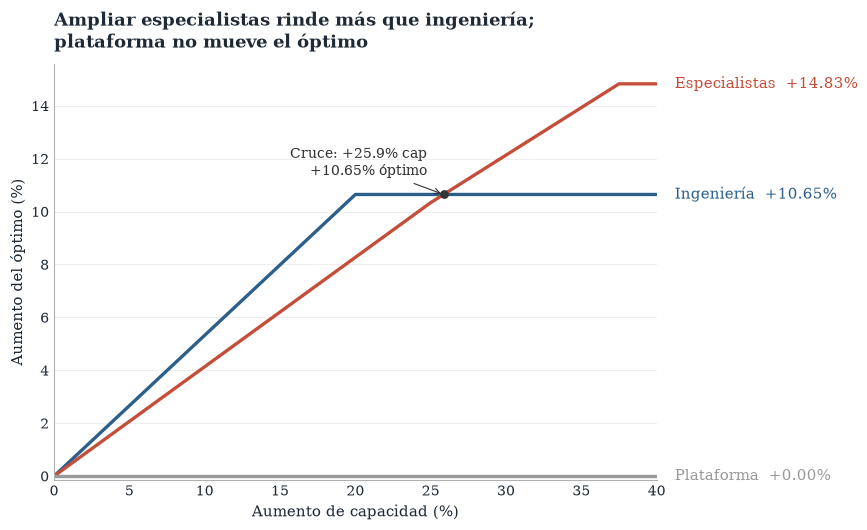
\includegraphics[width=0.78\textwidth]{report_assets/01_sensitivity_compare.png}
\caption{Ampliaciones independientes: especialistas rinde más en expansiones grandes; plataforma no aporta.}
\label{fig:sens1}
\end{figure}

\resultado{Ingeniería rinde más al inicio y se agota cerca de $+20\%$. Especialistas alcanza $\approx +14{,}8\%$ del óptimo y deja de aportar cerca de $+37{,}5\%$. Plataforma: $+0\%$. Cruce cerca de $+25{,}9\%$: por debajo conviene más ingeniería; por encima, especialistas.}

\interpretacion{Para expansiones pequeñas, ingeniería responde antes; para expansiones mayores, especialistas aporta más valor total. Ampliar plataforma no mueve el óptimo en el rango evaluado. Detalle del valor y del mix por recurso: Figura~\ref{fig:sens2}.}

\verif{Umbrales obtenidos en grilla numérica (paso $\approx 0{,}5\%$). Precios sombra son locales, no constantes globales.}

\clearpage
\begin{figure}[p]
\centering
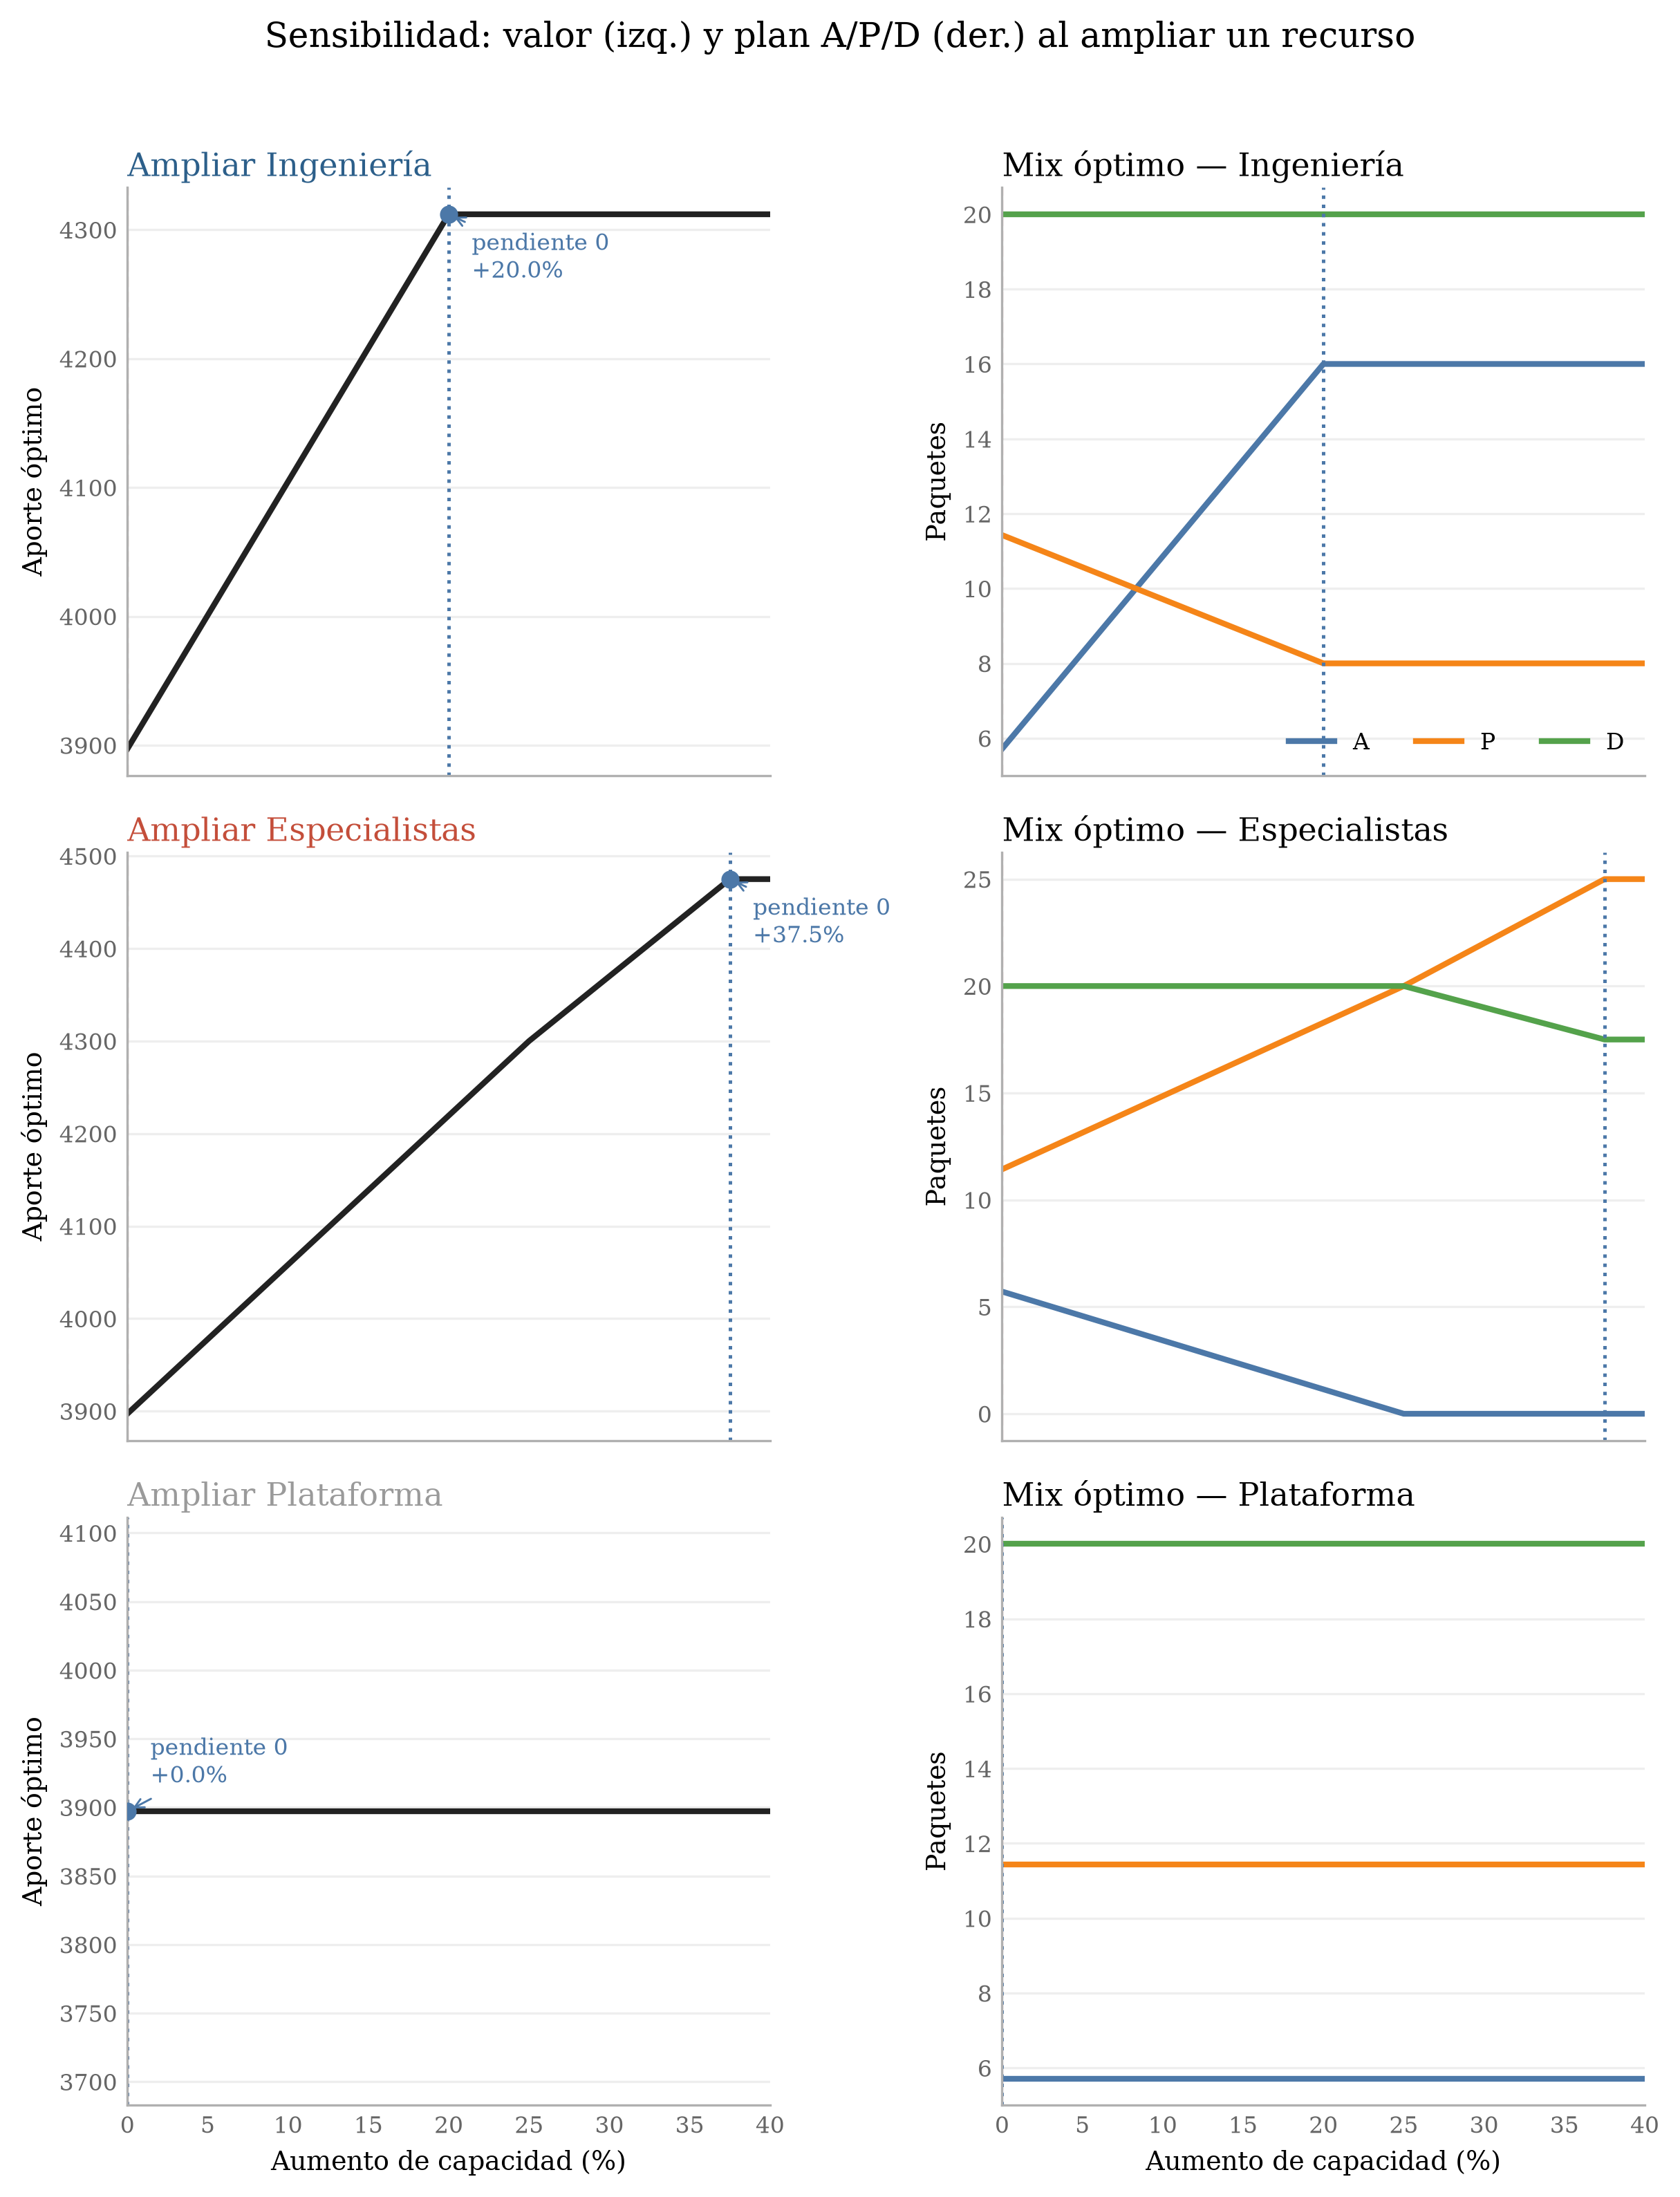
\includegraphics[width=\textwidth,height=0.92\textheight,keepaspectratio]{report_assets/01_sensitivity_panels.png}
\caption{Valor óptimo (izquierda) y mix $A/P/D$ (derecha) por fila de ampliación: ingeniería, especialistas y plataforma.}
\label{fig:sens2}
\end{figure}
\clearpage

%==============================================================================
\section{Dónde genera valor ampliar capacidad}
%==============================================================================

\pregunta{Ante ampliaciones discretas de $+10$ unidades, ¿qué recurso genera más impacto?}

\subsection*{Modelo}
Mismo LP del §1. Seis vectores independientes (no acumulativos); solo cambian los lados derechos; cada escenario se reoptimiza desde cero.

\subsection*{Resultado}

\begin{table}[H]
\centering
\small
\caption{Seis escenarios de capacidad.}
\label{tab:esc}
\begin{tabular}{@{}lcccc@{}}
\toprule
Escenario & Plan $(A,P,D)$ & $Z$ & $\Delta$ vs base & Activas \\
\midrule
Base $(120,80,100)$ & $(5{,}71;\,11{,}43;\,20)$ & $3\,897$ & $0$ & Ing, Esp, $D$ \\
$+10$ Ingeniería & $(10;\,10;\,20)$ & $4\,070$ & $+173$ & Ing, Esp, $D$ \\
$+10$ Especialistas & $(2{,}86;\,15{,}71;\,20)$ & $4\,099$ & $+201$ & Ing, Esp, $D$ \\
$+10$ Plataforma & $(5{,}71;\,11{,}43;\,20)$ & $3\,897$ & $0$ & Ing, Esp, $D$ \\
$+10$ Ing $+10$ Esp & $(7{,}14;\,14{,}29;\,20)$ & $4\,271$ & $+374$ & Ing, Esp, $D$ \\
Ampliado $(140,100,120)$ & $(8{,}57;\,17{,}14;\,20)$ & $4\,646$ & $+749$ & Ing, Esp, $D$ \\
\bottomrule
\end{tabular}
\end{table}

Interacción $+10$ Ing / $+10$ Esp:
\[
\Delta_{I}=172{,}86,\quad
\Delta_{E}=201{,}43,\quad
\Delta_{IE}=374{,}29,\quad
\Delta_{IE}-(\Delta_I+\Delta_E)\approx 0.
\]

\begin{figure}[H]
\centering
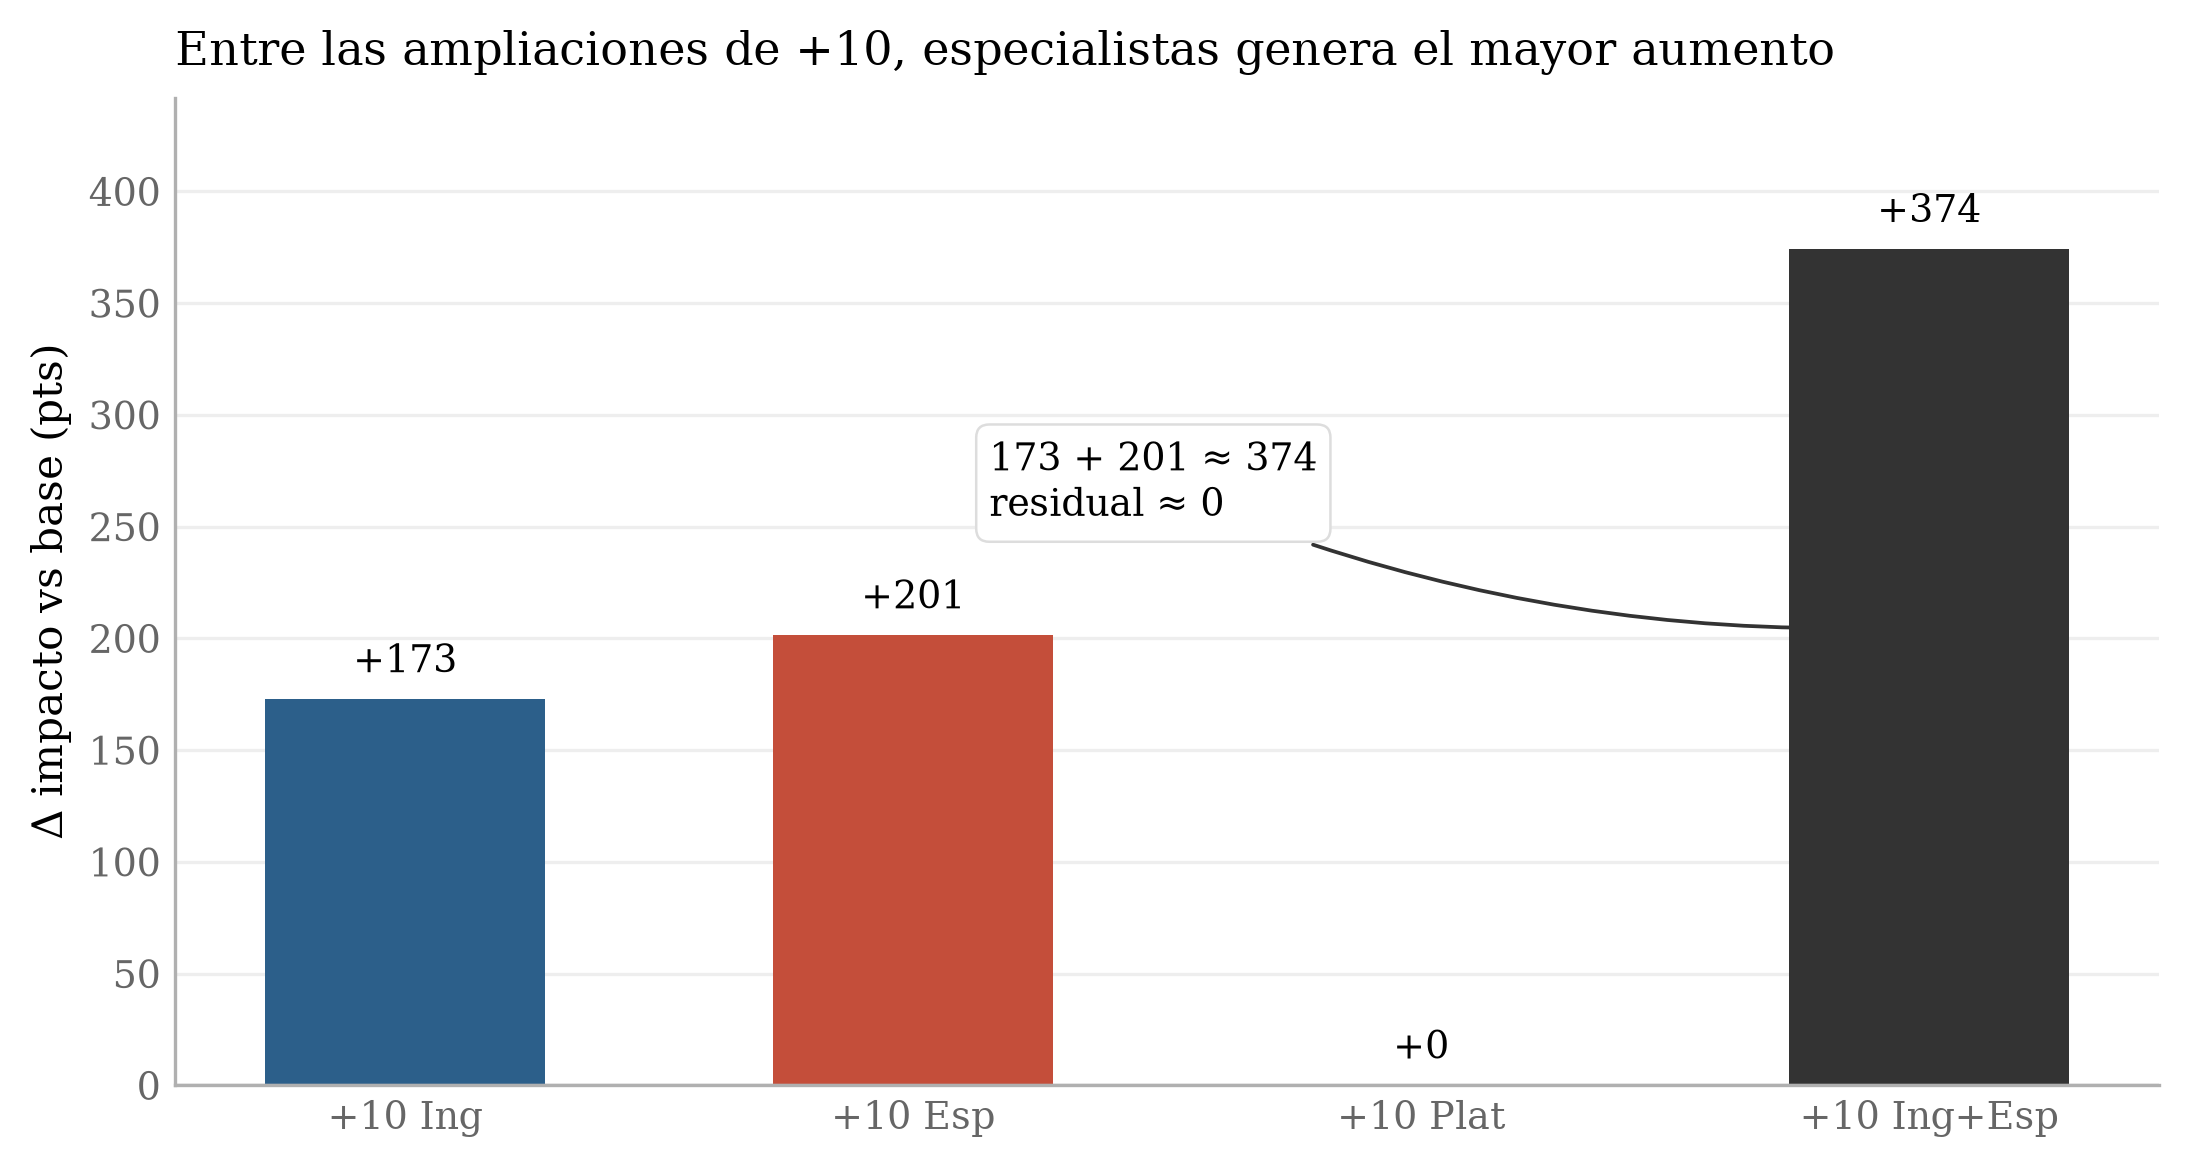
\includegraphics[width=0.76\textwidth]{report_assets/02_capacity_value.png}
\caption{Incrementos de $+10$: especialistas aporta más; plataforma no mueve $Z$.}
\label{fig:esc}
\end{figure}

\interpretacion{Si solo se puede ampliar un recurso en $+10$, especialistas es la mejor opción ($+201$ frente a $+173$). Ampliar solo plataforma no cambia nada. Ampliar ambos juntos suma $\approx 374$ pts, igual a la suma de los efectos individuales en esta combinación.}

\verif{Aditividad solo en el $+10/+10$ evaluado; no implica sinergia ni aditividad universal. Monotonicidad verificada en todos los pares con capacidades componente a componente $\ge$.}

%==============================================================================
\section{¿Conviene comprar capacidad al precio actual?}
%==============================================================================

\pregunta{¿Conviene adquirir capacidad externa a $12$ pts/u (ingeniería) y $16$ pts/u (especialistas)?}

\subsection*{Modelo}
Variables adicionales $e\in[0,20]$, $s\in[0,15]$ (continuas):
\begin{equation}
\max Z = 72A + 95P + 120D - 12e - 16s
\end{equation}
con $3A+2P+4D\le 120+e$, $A+3P+2D\le 80+s$ y plataforma fija en $100$. Comprar una unidad relaja la restricción (coeficiente $-1$ al pasar $e$ o $s$ al lado izquierdo).

\subsection*{Resultado}

\begin{table}[H]
\centering
\small
\caption{Sin compra frente a compra óptima.}
\label{tab:compra}
\begin{tabular}{@{}lcccccc@{}}
\toprule
 & Plan & $e$ & $s$ & Bruto & Costo & Neto \\
\midrule
Sin compra & $(5{,}71;\,11{,}43;\,20)$ & $0$ & $0$ & $3\,897$ & $0$ & $3\,897$ \\
Con compra & $(10;\,15;\,20)$ & $20$ & $15$ & $4\,545$ & $480$ & $4\,065$ \\
\bottomrule
\end{tabular}
\end{table}

Bruto $+648$; costo $480$ ($240$ Ing $+240$ Esp); neto $\approx +168$. Umbrales (reoptimización): compra deja de convenir cerca de $\approx 17{,}29$ (Ing) y $\approx 20{,}14$ (Esp).

\begin{figure}[H]
\centering
\begin{minipage}{0.48\textwidth}
\centering
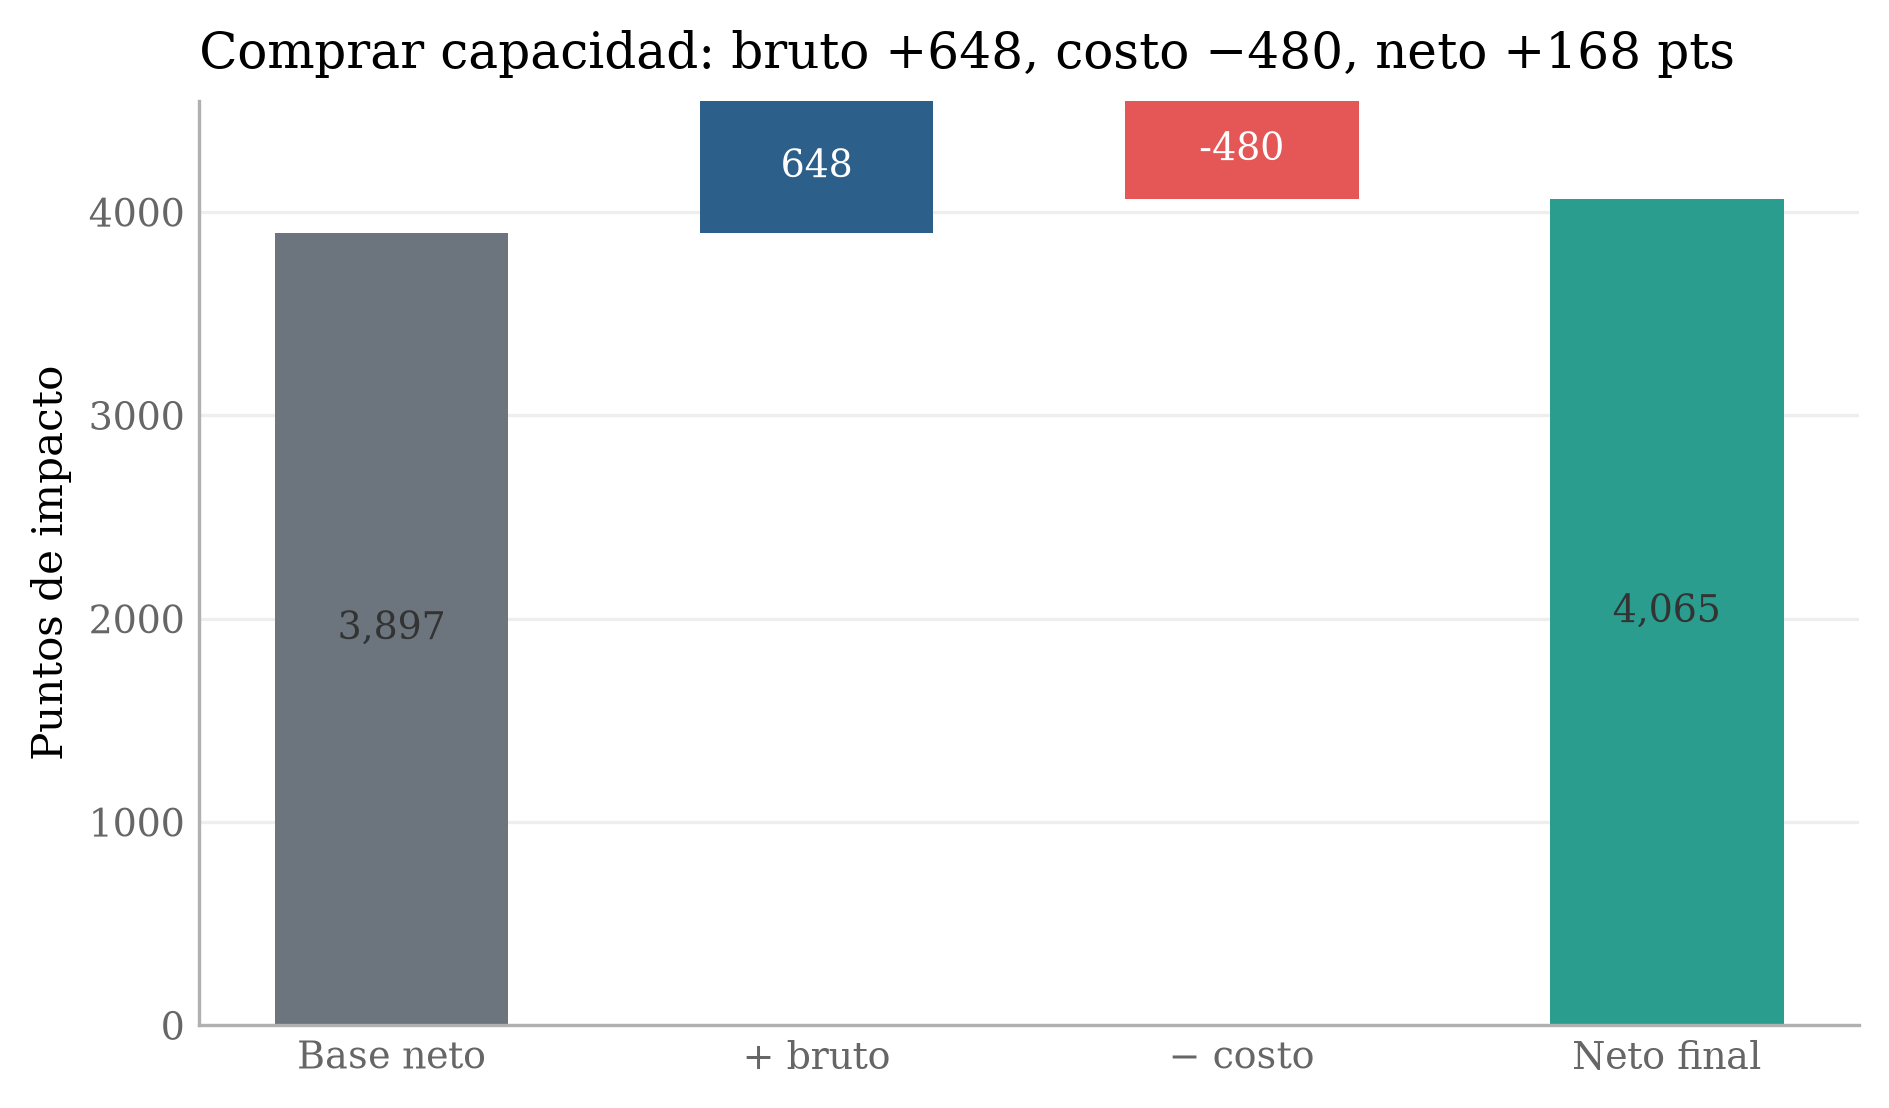
\includegraphics[width=\linewidth]{report_assets/03_capacity_purchase_waterfall.png}
\caption{Cascada: base $\to$ bruto $\to$ costo $\to$ neto.}
\label{fig:water}
\end{minipage}\hfill
\begin{minipage}{0.48\textwidth}
\centering
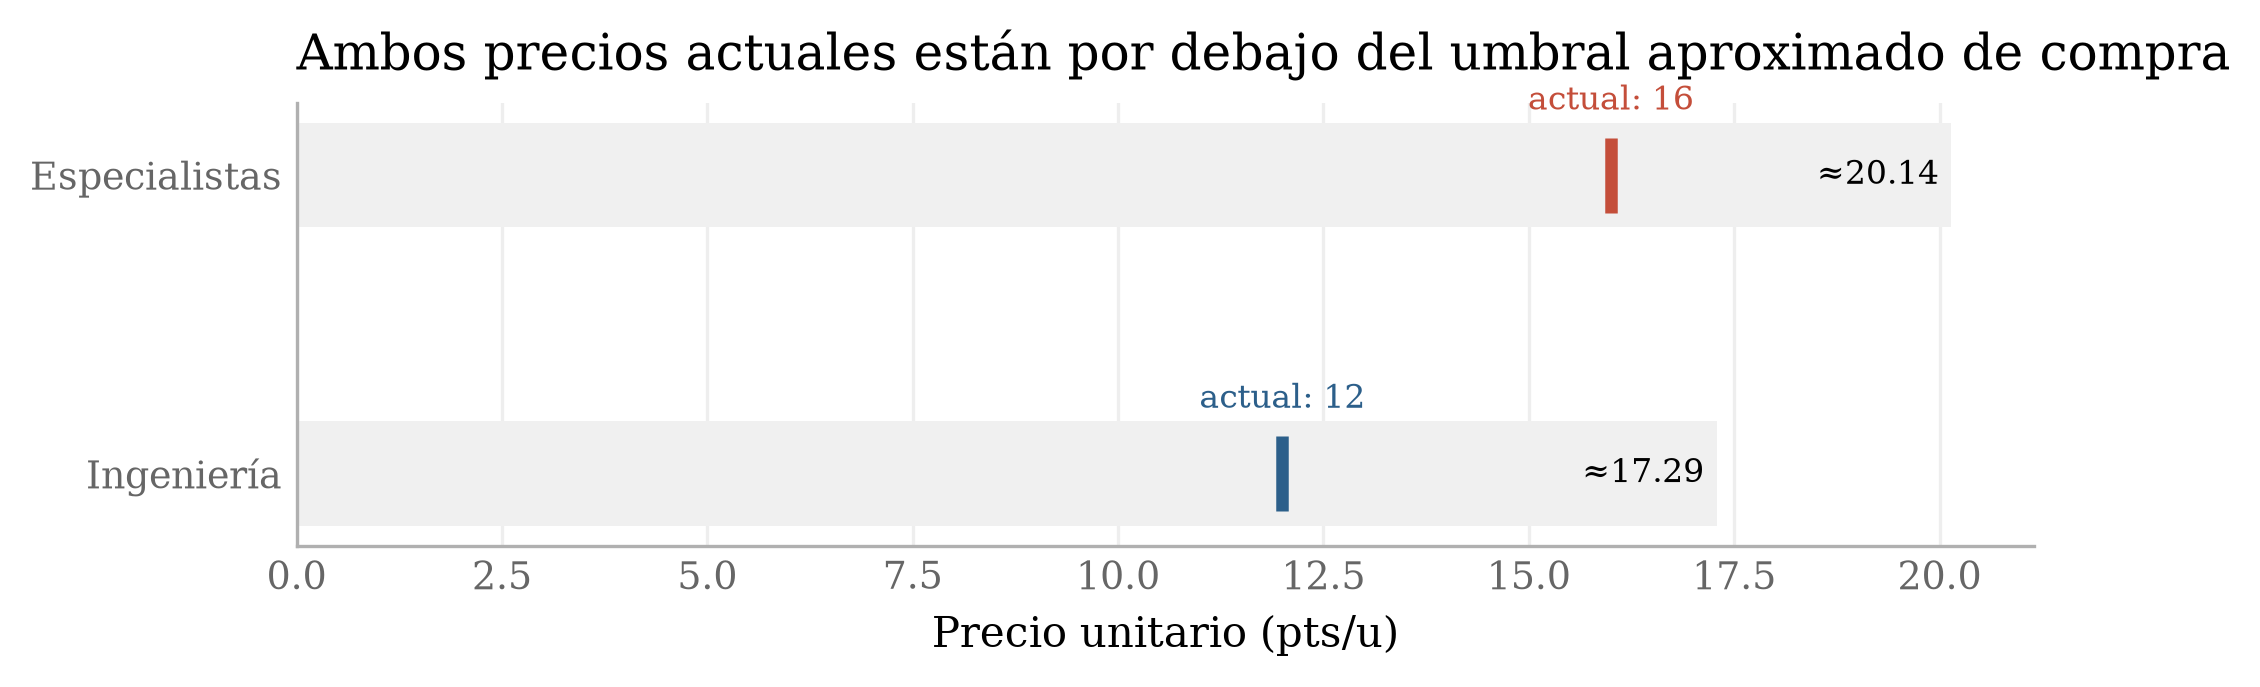
\includegraphics[width=\linewidth]{report_assets/03_purchase_thresholds.png}
\caption{Precios actuales bajo los umbrales.}
\label{fig:thr}
\end{minipage}
\end{figure}

\interpretacion{A los precios actuales, comprar al máximo ($e=20$, $s=15$) mejora el neto. El $+648$ bruto no es beneficio libre: tras el costo quedan $\approx +168$. Si el proveedor supera $\approx 17{,}3$ / $\approx 20{,}1$, conviene recomputar.}

\verif{Controles: $e=s=0$ reproduce la base; costos prohibitivos $\Rightarrow e=s=0$ y plan base. Umbrales coherentes con precios sombra locales (no globales). Si la compra fuera por bloques o con cargo fijo, haría falta un MILP.}

%==============================================================================
\section{Cuánto cuesta comprometer el plan antes de conocer la capacidad}
%==============================================================================

\pregunta{Si el mix debe fijarse hoy, ¿cuánto se sacrifica frente a adaptar el plan con información perfecta?}

\subsection*{Modelo}
Un único $(A,P,D)$ factible en
\[
S1=(120,80,100),\quad
S2=(110,90,95),\quad
S3=(130,70,105),
\]
apilando las nueve restricciones de recursos. Sin probabilidades ni valor esperado. Planes adaptados = referencia con información perfecta --- no implementable hoy.

\subsection*{Resultado}
\[
(A,P,D)\approx(4{,}29;\;8{,}57;\;20),\qquad Z\approx 3\,522{,}86.
\]
Brechas: $S1$ $+374$ ($9{,}6\%$); $S2$ $+390$ ($10{,}0\%$); $S3$ $+346$ ($8{,}9\%$). En el óptimo robusto: S2 activa ingeniería; S3 activa especialistas; plataforma con holgura en los tres escenarios.

\begin{figure}[H]
\centering
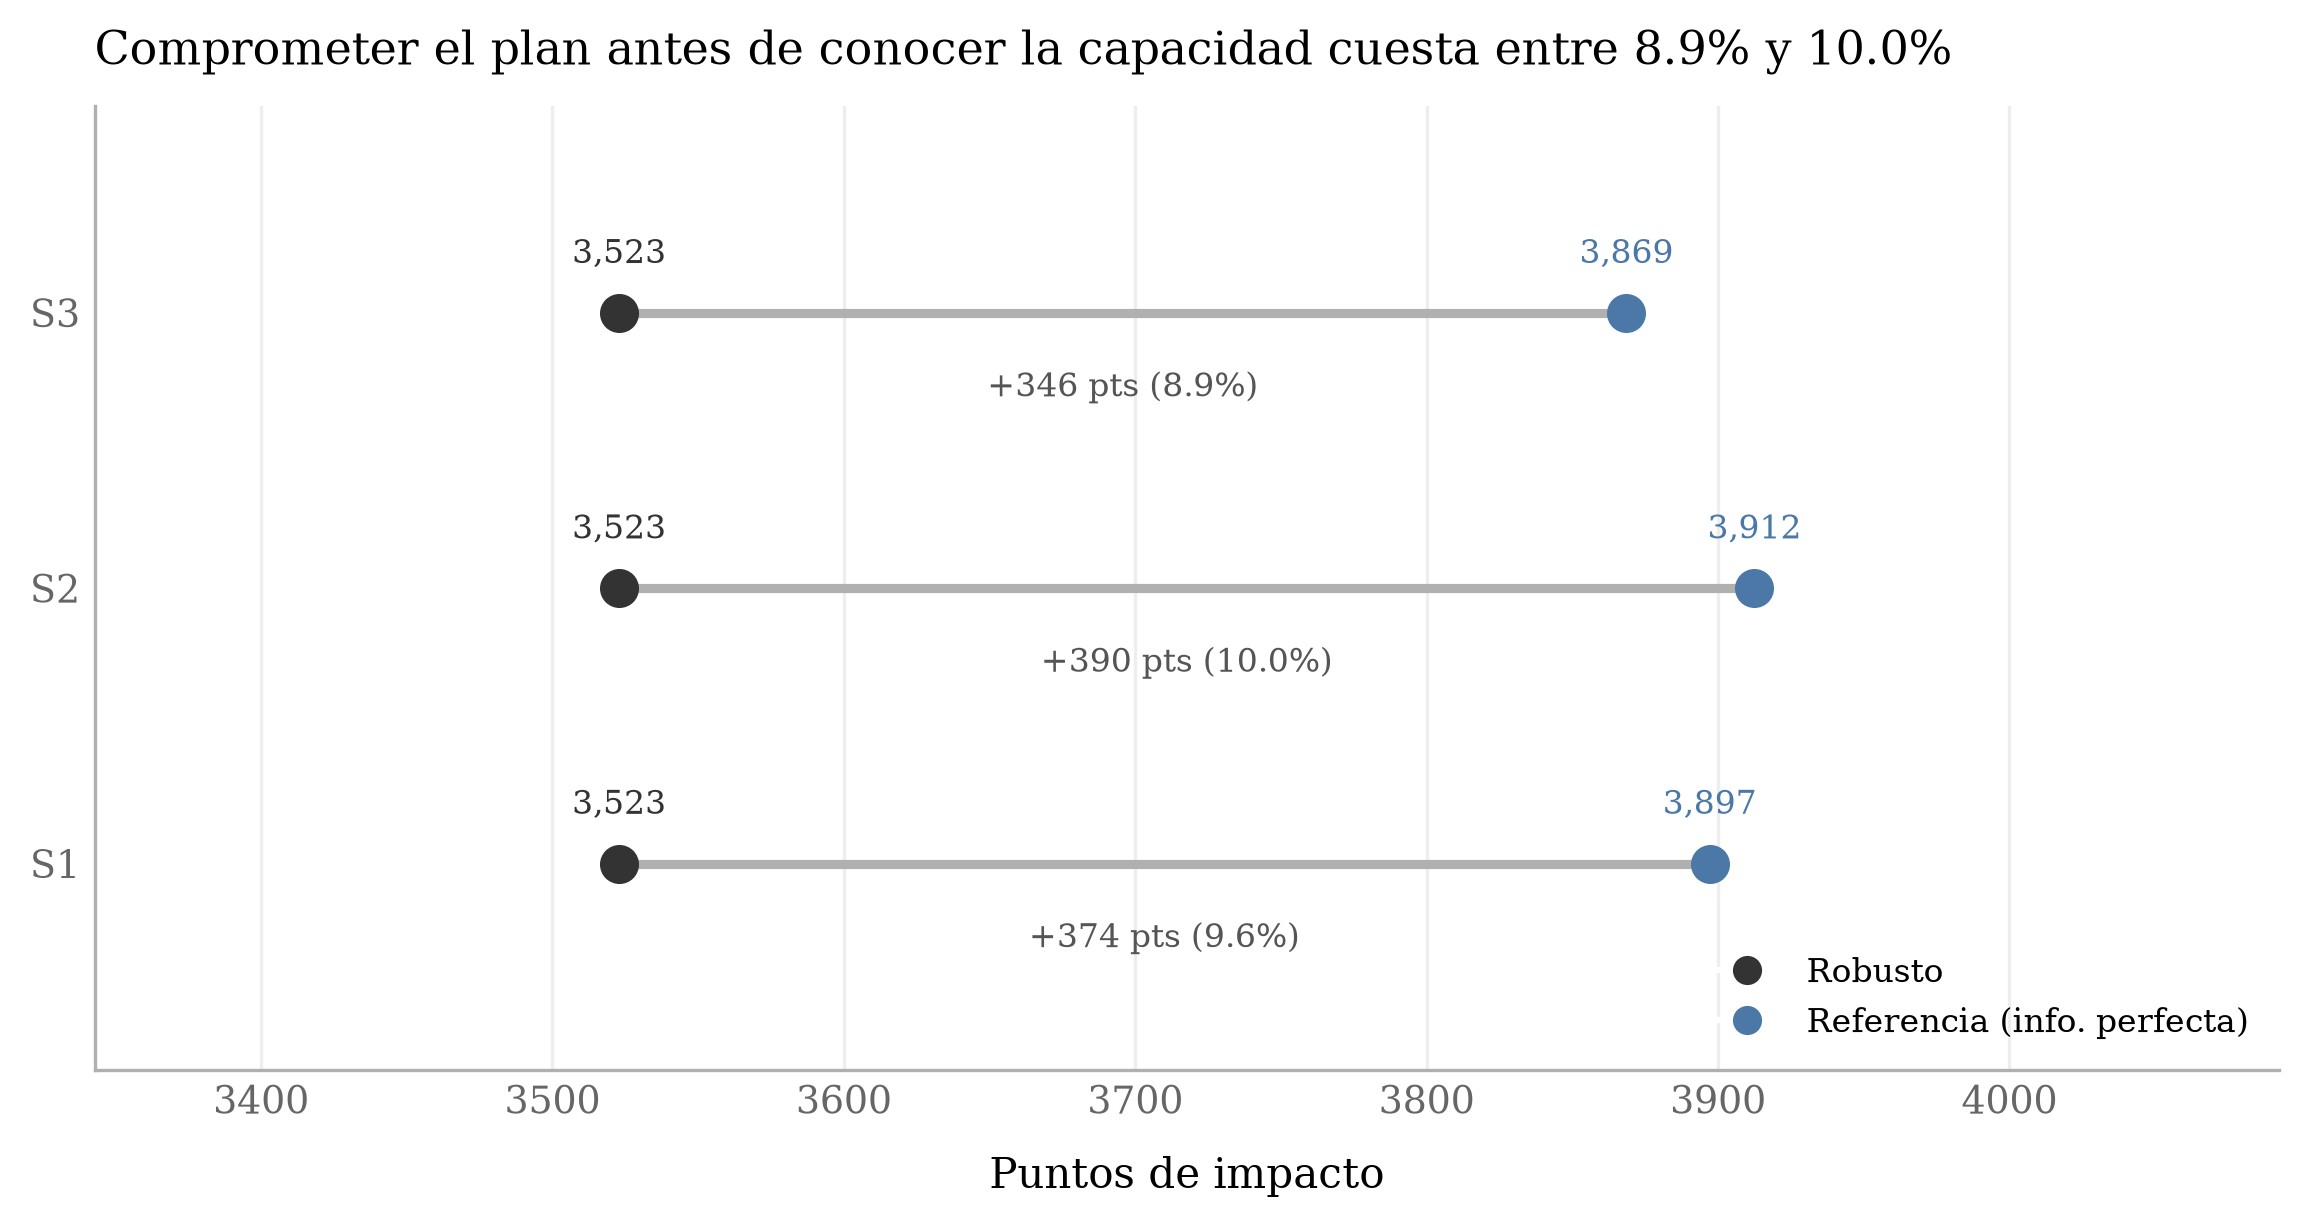
\includegraphics[width=0.80\textwidth]{report_assets/04_robust_gap.png}
\caption{Plan robusto vs.\ referencias perfectas. Costo del compromiso: $\approx 8{,}9$--$10{,}0\%$.}
\label{fig:rob}
\end{figure}

\interpretacion{Fijar el mix antes de observar la capacidad cuesta del orden de una décima parte del impacto adaptativo. A cambio, el plan es factible en los tres escenarios modelados.}

\verif{Los vectores no están totalmente ordenados: no se afirma que $S2$ sea ``el más restrictivo'' en sentido global. Plan $(0,0,0)$ factible; las nueve desigualdades se verifican con el plan robusto.}

%==============================================================================
\section{Síntesis}
%==============================================================================

\begin{table}[H]
\centering
\small
\caption{Resumen de los tres modelos.}
\label{tab:sint}
\begin{tabularx}{\textwidth}{@{}lXXX@{}}
\toprule
Problema & Resultado & Mecanismo & Límite \\
\midrule
Reoptimización & $+10$ Esp ($+201$) $> +10$ Ing ($+173$); Plat $=0$ & Ing y Esp activas en base & Aditividad solo en $+10/+10$ \\
Compra & $e=20$, $s=15$; neto $+168$ & Precios $<$ umbrales locales & Costos lineales; productividad homogénea \\
Robusto & $(4{,}29;\,8{,}57;\,20)$; brecha $8{,}9$--$10\%$ & S2$\to$Ing; S3$\to$Esp & Tres escenarios; sin adaptación ex post \\
\bottomrule
\end{tabularx}
\end{table}

\subsection*{Conclusiones}
\begin{enumerate}
\item Los cuellos de botella son ingeniería y especialistas; ampliar plataforma no genera valor en el rango evaluado.
\item Conviene comprar al precio contractual: neto $\approx +168$ tras descontar $480$ de costo.
\item Un plan robusto sacrifica $\approx 9$--$10\%$ frente a reoptimizar con información perfecta.
\end{enumerate}

\subsection*{Supuestos a validar}
\begin{itemize}
\item Divisibilidad de paquetes y de capacidad comprada.
\item Consumo e impacto lineales y comparables en puntos.
\item Demandas estables; costos de compra lineales, sin cargo fijo ni bloques.
\item Igual productividad interna/externa; sin inventario de capacidad no usada.
\item Completitud de los tres escenarios e imposibilidad de adaptar el plan ex post.
\end{itemize}

\vspace{0.5em}
\noindent\small\textit{Solver:} OR-Tools GLOP. \textit{Tolerancia:} $10^{-6}$. Validaciones: reconstrucción del objetivo, factibilidad, monotonicidad, controles de compra y verificación de las nueve restricciones robustas.

\end{document}
